\documentclass[tikz,border=1mm,12pt]{standalone}
%\usepackage[dvipsnames]{xcolor}
\usepackage{pgfplots}
\pgfplotsset{compat=1.5.1}
\usetikzlibrary{arrows}
\usetikzlibrary{patterns}


\newcommand{\W}{\mathcal{W}}

\begin{document}

	\tikzset{>=stealth',}

   	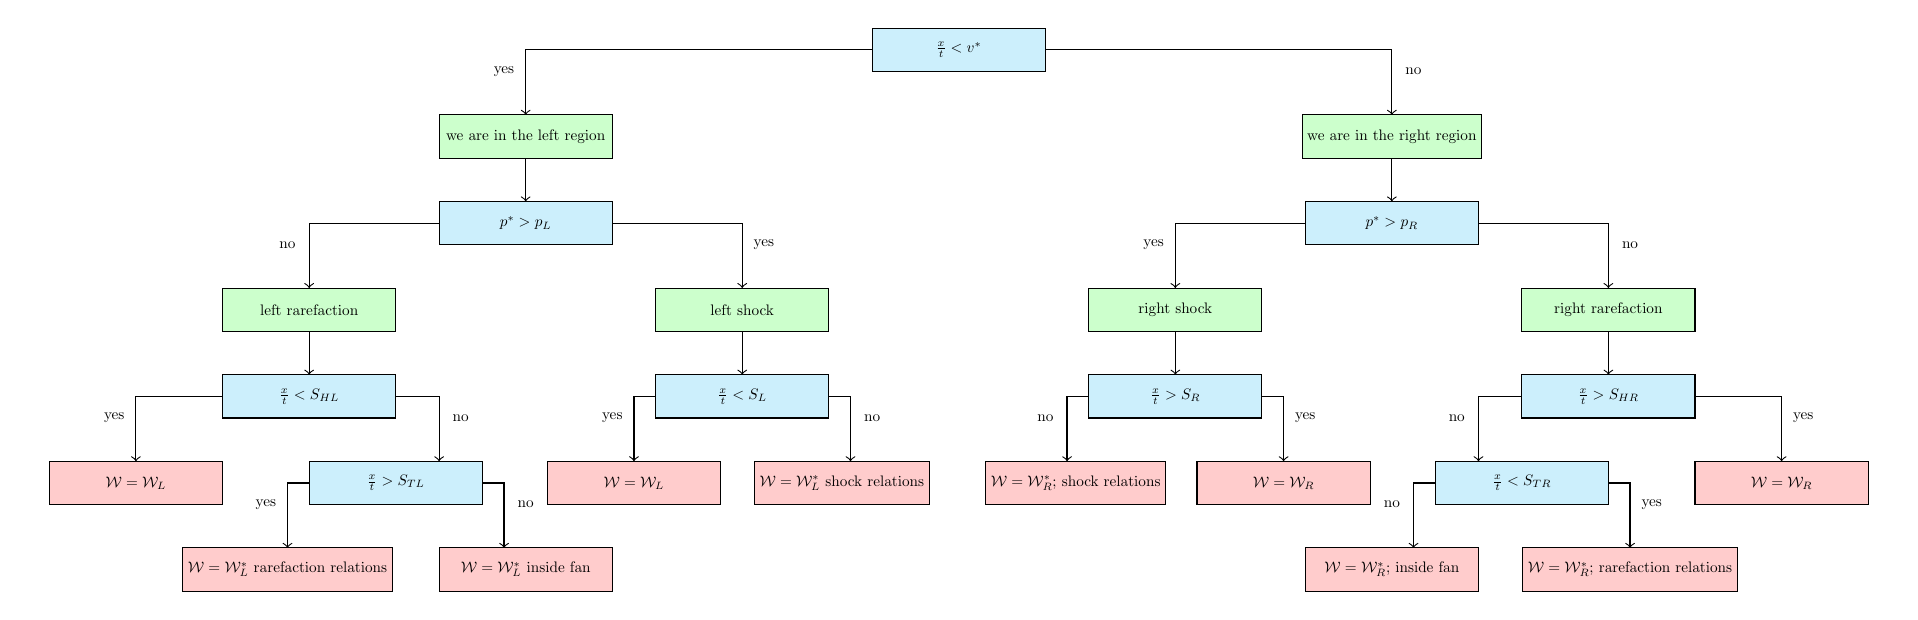
\begin{tikzpicture}[scale=0.55, every node/.style={scale=0.55, minimum height = 1cm, minimum width=4cm}]
   		
   		\node[draw, fill=cyan!20] at (0,10) {$\frac{x}{t} < v^*$};

	   	\draw[->] (-2,10) -- (-10,10)-- (-10, 8.5);
	   	\node at (-10.5, 9.5) {yes};
   		\node[draw, fill=green!20] at (-10,8) {we are in the left region};
   		
	   	\draw[->] (2,10) -- (10,10)-- (10, 8.5);
	   	\node at (10.5, 9.5) {no};
   		\node[draw, fill=green!20] at (10,8) {we are in the right region};
   		
   		
   		% LEFT SIDE
   		\draw[->] ( -10, 7.5) -- (-10, 6.5);
   		\node[draw, fill=cyan!20] at (-10, 6) {$p^* > p_L$};
   		
   		\draw[->] (-12, 6) -- (-15, 6) -- (-15, 4.5);
   		\node at (-15.5, 5.5) {no};
   		\node[draw, fill=green!20] at (-15, 4) {left rarefaction};
   		
   		\draw[->] (-15, 3.5) -- (-15, 2.5);
   		\node[draw, fill=cyan!20] at (-15, 2) {$\frac{x}{t} < S_{HL}$};
   		
   		\draw[->] (-17, 2) -- (-19, 2) -- (-19, 0.5);
   		\node at (-19.5, 1.5) {yes};
   		\node[draw, fill=red!20] at (-19, 0) {$\W = \W_L$};
   		
   		\draw[->] (-13, 2) -- (-12, 2) -- (-12, 0.5);
   		\node at (-11.5, 1.5) {no};
   		\node[draw, fill=cyan!20] at (-13, 0) {$ \frac{x}{t} > S_{TL}$};
   		
   		\draw[->] (-15, 0) -- (-15.5, 0) -- (-15.5, -1.5);
   		\node at (-16, -0.5) {yes};
   		\node[draw, fill=red!20] at (-15.5, -2) {$\W = \W^*_L$ rarefaction relations};
   		
   		\draw[->] (-11, 0) -- (-10.5, 0) -- (-10.5, -1.5);
   		\node at (-10, -0.5) {no};
   		\node[draw, fill=red!20] at (-10., -2) {$\W = \W^*_L$ inside fan};
   		
   		
   		
   		\draw[->] (-8, 6) -- (-5, 6) -- (-5, 4.5);
   		\node at (-4.5, 5.5) {yes};
   		\node[draw, fill=green!20] at (-5, 4) {left shock};
   		
   		\draw[->] (-5, 3.5) -- (-5, 2.5);
   		\node[draw, fill=cyan!20] at (-5, 2) {$\frac{x}{t} < S_L$};
   		
   		\draw[->] (-7, 2) -- (-7.5, 2) -- (-7.5, 0.5);
   		\node at (-8, 1.5) {yes};
   		\node[draw, fill=red!20] at (-7.5, 0) {$\W = \W_L$};
   		
   		\draw[->] (-3, 2) -- (-2.5, 2) -- (-2.5, 0.5);
   		\node at (-2, 1.5) {no};  		
   		\node[draw, fill=red!20] at (-2.7, 0) {$\W = \W_L^*$ shock relations};
   		



   		% RIGHT SIDE
   		\draw[->] ( 10, 7.5) -- (10, 6.5);
   		\node[draw, fill=cyan!20] at (10, 6) {$p^* > p_R$};
   		
   		\draw[->] (12, 6) -- (15, 6) -- (15, 4.5);
   		\node at (15.5, 5.5) {no};
   		\node[draw, fill=green!20] at (15, 4) {right rarefaction};
   		
   		\draw[->] (15, 3.5) -- (15, 2.5);
   		\node[draw, fill=cyan!20] at (15, 2) {$\frac{x}{t} > S_{HR}$};
   		
   		\draw[->] (17, 2) -- (19, 2) -- (19, 0.5);
   		\node at (19.5, 1.5) {yes};
   		\node[draw, fill=red!20] at (19, 0) {$\W = \W_R$};
   		
   		\draw[->] (13, 2) -- (12, 2) -- (12, 0.5);
   		\node at (11.5, 1.5) {no};
   		\node[draw, fill=cyan!20] at (13, 0) {$ \frac{x}{t} < S_{TR}$};
   		
   		\draw[->] (15, 0) -- (15.5, 0) -- (15.5, -1.5);
   		\node at (16, -0.5) {yes};
   		\node[draw, fill=red!20] at (15.5, -2) {$\W = \W^*_R$; rarefaction relations};
   		
   		\draw[->] (11, 0) -- (10.5, 0) -- (10.5, -1.5);
   		\node at (10, -0.5) {no};
   		\node[draw, fill=red!20] at (10., -2) {$\W = \W^*_R$; inside fan};
   		
   		
   		
   		\draw[->] (8, 6) -- (5, 6) -- (5, 4.5);
   		\node at (4.5, 5.5) {yes};
   		\node[draw, fill=green!20] at (5, 4) {right shock};
   		
   		\draw[->] (5, 3.5) -- (5, 2.5);
   		\node[draw, fill=cyan!20] at (5, 2) {$\frac{x}{t} > S_R$};
   		
   		\draw[->] (7, 2) -- (7.5, 2) -- (7.5, 0.5);
   		\node at (8, 1.5) {yes};
   		\node[draw, fill=red!20] at (7.5, 0) {$\W = \W_R$};
   		
   		\draw[->] (3, 2) -- (2.5, 2) -- (2.5, 0.5);
   		\node at (2, 1.5) {no};  		
   		\node[draw, fill=red!20] at (2.7, 0) {$\W = \W_R^*$; shock relations};
   	\end{tikzpicture}

\end{document}
